\documentclass[12pt]{article}

%============================================
%============================================
%===== PACKAGES AND DOCUMENT SETTINGS =====
%============================================
%============================================

%===== General margin setup =====
\setlength{\oddsidemargin}{0.25 in}
\setlength{\evensidemargin}{-0.25 in}
\setlength{\topmargin}{-0.6 in}
\setlength{\textwidth}{6.5 in}
\setlength{\textheight}{8.5 in}
\setlength{\headsep}{0.75 in}
\setlength{\parindent}{0 in}
\setlength{\parskip}{0.1 in}

%===== Packages that I normally like to use
\usepackage{amsmath,amssymb} %General math symbols and stuff
\usepackage[mathscr]{euscript} %To use script letters with \mathscr{}
\usepackage{amsthm} %To be able to write Definitions, Theorems, etc.
\usepackage{graphicx} % To scale equation*s and put figures wherever
\usepackage{framed} % To be able to frame theorems and stuff with begin{framed} ... \end{framed}
\usepackage{float} %To be able to place figures exactly where I want with [H]
\usepackage{multirow}
\usepackage{color}
\usepackage{cite}
\usepackage[hidelinks, breaklinks=true]{hyperref} %To be able to use links inside the document; [hidelinks removes the ugly red boxes]
\usepackage{xcolor}  \definecolor{shadecolor}{rgb}{.95,.95,.95}  %To put a shaded region
%\usepackage[font=footnotesize]{caption}
\usepackage{nicefrac} %to put small fractions nicely with \nicefrac{1}{2}
\usepackage{ragged2e}	%to put \justify
\usepackage[shortlabels]{enumitem}	%To put letters in enumerate with begin{enumitem}[(a)]
\usepackage{amsmath}
\usepackage{amssymb}
\usepackage[super]{nth}
%===== Algorithm setup =====
\usepackage[ruled,vlined]{algorithm2e}
\usepackage{graphicx}
\graphicspath{ {images/} }

%===== Example setup =====
\usepackage{mdframed}
\usepackage{changepage}
\newmdenv[
  topline=false,
  bottomline=false,
  skipabove=\topsep,
  skipbelow=\topsep
]{siderules}

%===== Theorems, lemmas, definitions, etc.
\theoremstyle{definition}
\newtheorem{myDefinition}{Definition}
\newtheorem{myTheorem}{Theorem}
\newtheorem{myLemma}{Lemma}
\newtheorem{myCorollary}{Corollary}
\newtheorem{myProposition}{Proposition}
\newtheorem{myExample}{Example}
\newtheorem{myExercise}{Exercise}
\newtheorem{myRemark}{Remark}
\newtheorem{myConjecture}{Conjecture}

%===== Page counters, theorem counters, etc.
\newcounter{lecnum}
\renewcommand{\thepage}{\thelecnum-\arabic{page}}
\renewcommand{\thesection}{\thelecnum.\arabic{section}}
\renewcommand{\theequation}{\thelecnum.\arabic{equation}}
\renewcommand{\thefigure}{\thelecnum.\arabic{figure}}
\renewcommand{\thetable}{\thelecnum.\arabic{table}}
\renewcommand{\themyDefinition}{\thelecnum.\arabic{myDefinition}}
\renewcommand{\themyTheorem}{\thelecnum.\arabic{myTheorem}}
\renewcommand{\themyLemma}{\thelecnum.\arabic{myLemma}}
\renewcommand{\themyCorollary}{\thelecnum.\arabic{myCorollary}}
\renewcommand{\themyProposition}{\thelecnum.\arabic{myProposition}}
\renewcommand{\themyExample}{\thelecnum.\arabic{myExample}}
\renewcommand{\themyExercise}{\thelecnum.\arabic{myExercise}}
\renewcommand{\themyRemark}{\thelecnum.\arabic{myRemark}}
\renewcommand{\themyConjecture}{\thelecnum.\arabic{myConjecture}}

%===== Header box =====
\newcommand{\lecture}[3]{
\pagestyle{myheadings}
\thispagestyle{plain}
\newpage
\setcounter{lecnum}{#1}
\setcounter{page}{1}
\noindent
\begin{center}
\rule{\textwidth}{1.6pt}\vspace*{-\baselineskip}\vspace*{2pt} % Thick horizontal line
\rule{\textwidth}{0.4pt}\\[1\baselineskip] % Thin horizontal line
\vbox{\vspace{2mm}
\hbox to 6.28in { {\bf CS 4980/6980: Predictive Data Analysis } \hfill $\copyright$ Spring 2018 }
\vspace{4mm}
\hbox to 6.28in { {\Large \hfill Lecture #1: #2  \hfill} }
\vspace{4mm}
\hbox to 6.28in { {\scshape Instructor: Daniel L. Pimentel-Alarc\'on}   \hspace{3mm}\hfill Scribed by: #3 }}
\vspace{-2mm}
\rule{\textwidth}{0.4pt}\vspace*{-\baselineskip}\vspace{3.2pt} % Thin horizontal line
\rule{\textwidth}{1.6pt}\\[\baselineskip] % Thick horizontal line
\end{center}
\markboth{Lecture #1: #2}{Lecture #1: #2}
\vspace*{4mm}
}

%====================================
%====================================
% ===== VARIABLES AND COMMANDS =====
%====================================
%====================================


%===== Some frequent commands that I use =====
\newcommand{\bs}[1]{\boldsymbol{#1}} %bold symbol
\newcommand{\hatt}[1]{\boldsymbol{\hat{#1}}} %bold hat
\newcommand{\careful}{\textcolor{red}}
\newcommand{\comment}{\textcolor{blue}}
\newcommand*\rot{\rotatebox{90}} %To rotate text in table
\newcommand*{\Scale}[2][4]{\scalebox{#1}{\ensuremath{#2}}} % To scale variables in equation*s
\newcommand\tab[1][1.25cm]{\hspace*{#1}}
%===== In case you want to add colored text =====
\newcommand{\blue}{\textcolor{blue}}

%===== Miscelaneous math symbols =====
\def \R{\mathbb{R}}
\def \Pr{\mathsf{P}}
\def \T{\mathsf{T}}
\def \c{\mathsf{c}}
\def \spn{{\rm span}}
\def \Ord{\mathscr{O}}
\def \<{\langle}
\def \>{\rangle}
\DeclareMathOperator*{\argmin}{arg\,min}
\DeclareMathOperator*{\argmax}{arg\,max}

%===== Common scalars that will be used throughout =====
\def \D{{\hyperref[DDef]{{\rm D}}}} % ambient Dimension
\def \N{{\hyperref[NDef]{{\rm N}}}} %Number of samples
\def \xi{{\hyperref[xiDef]{{\rm x}}}} % a scalar variable x

%===== Common vectors that will be used throughout =====
\def \xx{{\hyperref[xxDef]{\bs{{\rm x}}}}} % a vector x
\def \yy{{\hyperref[yyDef]{\bs{{\rm y}}}}} % a vector y

%===== Common matrices that will be used throughout =====
\def \I{{\hyperref[IDef]{\bs{{\rm I}}}}} % Identity matrix
\def \X{{\hyperref[XDef]{\bs{{\rm X}}}}} % Data matrixm

%Indices that will be used throughout.
%\newcommand{\R}{\mathbb{R}}
\def \i{{\hyperref[iDef]{{\rm i}}}} % index used for samples, usually goes from 1 to N

%=====================================
%=====================================
%===== HERE BEGINS THE DOCUMENT =====
%=====================================
%=====================================

\begin{document}
%===== Lecture's number, title, and students' names.
\lecture{20} % Lecture number
{Vector Spaces and Linear Combinations} % Lecture title
{Naman Kanwar} % Students' name
%===== Section
\section{Introduction}
A \textbf{Vector Space} \textit{informally} is a set of objects (vectors or points) that can be added and multiplied without \textbf{"falling"} outside of the set.\\
\\
\textit{Falling Outside of set} : A point or vector does not qualify to be an element of the set. For example:\\

Suppose $\R_{+}$ := \{Set of all positive numbers\}
\begin{center}
Then: 5 $\in \R_{+}$\\
\tab 7 $\in \R_{+}$ \\
5 -7= -2 $\notin \R_{+}$\\
Therefore, -2 fall outside of set and $\R_{+}$ is not a \textbf{Vector Space}  
\end{center}  

\section{Vector Space}
\textbf{A Formal Definition of a Vector Space}\\
A set $\mathscr{V}$ is a vector space if $\forall v,w \in$ \textit{V}, and for every scalar values $a,b \in \R$\\
\begin{center}
a\textit{V} + b\textit{V} $\in $ \textit{V}
\end{center}  

\begin{figure}[H]
	\centering
	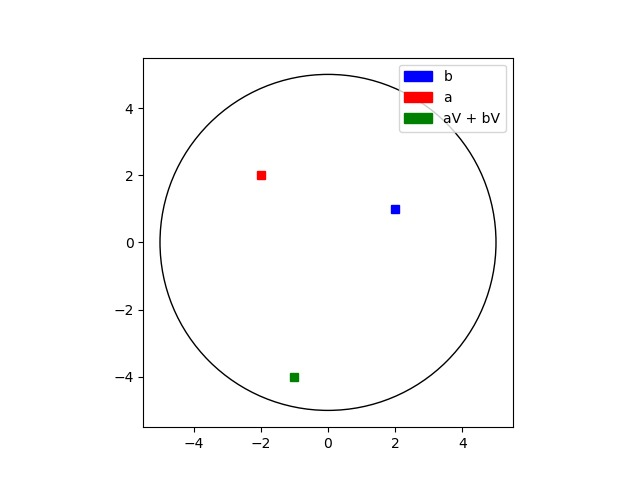
\includegraphics[width=0.7\linewidth, scale=0.7]{Figure_1.jpg}
	\caption{Looking at the nearest point only, the new point is classified as green.}
\end{figure}

A set $\mathscr{V}$ is also a vector space, if it is closed under linear combination (Will be discussed later).\\\\


Now the question arises:\\
Is $\R$ a vector space?\\
\begin{proof}
	$\R$ is a Vector Space\\
	\tab Let v, w $\in \R$\\
	\tab Let a, b  be scalars \tab every scalar a, b $\in \mathbb{K}$ \\
	\tab Let u = a$\mathscr{V}$ + b$\mathscr{V}$ $\in \R$\\
	\tab Then u $\in \R$	 
\end{proof}
\textbf{Some Examples:}\\\\
\textbf{\underline{Example 1:}} If \textit{W} = $\R$. Is $\mathbb{W}$ under $\sqrt{*}$\\
\tab \underline{Answer:} No, here's a a counter example:\begin{center}
-4 $\in \mathbb{W}$\\
$\sqrt{-4} = 2\iota \notin \mathbb{W}$
\end{center} 

\textbf{\underline{Example 2:}} If $\mathbb{W}$ = $\mathbb{Z}$ and $\mathbb{K}$ = $\R$. Is $\mathscr{V}$ a vector space?\\
\tab \underline{Answer:} No, here's a a counter example:\begin{center}
Take v = 1 and w = 2 $\in \mathbb{V}$\\
Take a= 0.5 and b= 0.5 $\in \mathbb{K}$\\
Let u = av + bw\\
u= 1.5 $\in \mathbb{V} \notin \R$
\end{center} 

\section{More about Vector Space}
A vector space satisfies the following additive properties:\\\\
\textbf{(A1) Closure: }$\forall$ v,w $\in \mathbb{V}$,  v + w $\in \mathbb{V}$\\
\textbf{(A2) Commutativity: }$\forall$ v,w $\in \mathbb{V}$,  v + w = w + v\\
\textbf{(A3) Associativity: }$\forall$ u,v,w $\in \mathbb{V}$, (u + v) + w = u + (v + w)\\
\textbf{(A4) Additive Identity: }$\exists$ an element in $\mathbb{V}$, denoted by 0 $\mid$ v $\in \mathbb{V}$, v + 0 = v\\
\textbf{(A5) Additive Inverse: }$\forall$ v $\in \mathbb{V}$, $\exists!$ element in $\mathbb{V}$, denoted by -v $\mid$ v + (-v) = 0\\

\textbf{\underline{Example 3:}} If $\mathbb{V}$ = $\mathbb{N}$. Is $\mathbb{V}$ a vector space?\\
\tab \underline{Answer:} No, because of \textbf{(A5) Additive Inverse} property\\\\

A vector space also has the following multiplicative properties:\\
\textbf{(M1) Closure: }$\forall$ a $\in \mathbb{R}$, and $\forall$ v $\in \mathbb{V}$, av $ \in \mathbb{V}$\\
\textbf{(M2) Associativity: }$\forall$ a, b $\in \mathbb{R}$, and $\forall$ v $\in \mathbb{V}$, a(bv) = (ab)v\\
\textbf{(M3) $\nth{1}$Distributive Law: }$\forall$ a $\in \mathbb{R}$, and $\forall$ v, w $\in \mathbb{V}$, a(v+w) = av + aw\\


\textbf{(M4) $\nth{2}$Distributive Law: }$\forall$ a, b $\in \mathbb{R}$, and $\forall$ v, w $\in \mathbb{V}$, (a+b)v = av + bv\\
\textbf{(M5) Multiplicative Identity: }$\forall$ v $\in \mathbb{V}$, 1v= v\\

\textbf{\underline{Example 4:}} If $\mathbb{V}= \R^2$. Is $\mathbb{V}$ a vector space?\\
\begin{proof}
	$\mathbb{V}$ is a Vector Space\\
	\tab Let  $\mathbb{V}= \R^2$ and $\mathbb{K}= \R$\\
	\tab \textbf{(A1)} Let vectors v, w  $\in \R^2$ \\
	\tab Let u = v + w\\
	\tab Then u $\in \R^2$\\	 

\end{proof}

\textbf{\underline{Example 5:}} Prove if \textbf{(A2)} holds?\\
\begin{proof} 
Let v, w $\in \R^2$\\
\tab Let u = v + w = $\begin{bmatrix}
v_{1} + w_1\\
v_{2} + w_2\\
\end{bmatrix}$\\
$\begin{bmatrix}
v_{1} + w_1\\
v_{2} + w_2\\
\end{bmatrix}$ = $\begin{bmatrix}
w_1\\
w_2\\
\end{bmatrix}$ + $\begin{bmatrix}
v_{1}\\
v_{2}\\
\end{bmatrix}$ = w + v\\
\end{proof}
\section{Linear Combination}
Let $\mathbb{V}$ be a vector space\\
Let $\textbf{v}_1, \textbf{v}_2,... \textbf{v}_r \in \mathbb{V}$\\
We say that \textbf{u} is a linear combination of the $\textbf{v}_1, \textbf{v}_2,... \textbf{v}_r$ if:\\\\
$$\textbf{u} =\sum_{i=1}^r c_i v_i$$ \textbf{u} = $c_1 v_1 + c_2 v_2+ ... + c_r v_r$\\
\\For some scalars $c_1, c_2,...c_r $. In this case $c_1, c_2,...c_r $ are called the coefficients of the \textbf{u} w.r.t $\textbf{v}_1, \textbf{v}_2,... \textbf{v}_r$\\
\textbf{v} = $\begin{bmatrix}
1\\
0\\
0\\
\end{bmatrix}$
\textbf{w} = $\begin{bmatrix}
0\\
1\\
0\\
\end{bmatrix}$
\textbf{x} = $\begin{bmatrix}
0\\
0\\
1\\
\end{bmatrix}$\\\\
\\\textbf{u} = $\begin{bmatrix}
7\\
5\\
1\\
\end{bmatrix}$ = 7$\begin{bmatrix}
1\\
0\\
0\\
\end{bmatrix}$ + 5$\begin{bmatrix}
0\\
1\\
0\\
\end{bmatrix}$ + 1$\begin{bmatrix}
0\\
0\\
1\\
\end{bmatrix}$\\
\\\tab = 7v + 5w + 1x\tab\tab\tab $c_1 = 7$\tab$c_2 = 5$\tab$c_3 = 1$
\end{document}